\chapter{Realizácia riešenia}\label{chap:research}

V tejto kapitole je opísaný priebeh realizácie praktickej časti diplomovej práce. Postup sa vo veľkej miere držal navrhnutého riešenia, avšak počas vývoja došlo k malým doplnkom. Na prácu s výpočtovo zložitými operáciami sme mali k dispozícii školský server, ktorý má dve grafické karty NVIDIA GeForce RTX 3060, každá s 12 GB pamäte, CPU AMD Ryzen 9 5900X a 64 GB RAM. Na prihlásenia a vykonávanie príkazov na vzdialenom počítači bol použitý štandardný sieťový protokol. Prístup k serveru je zdieľaný medzi úzkou skupinou ľudí, preto bolo treba brať ohľad aj na druhých používateľov.

\section{Experimentálne meranie}

Pred začiatkom merania sme sa oboznámili s odporúčaniami uvedenými v používateľskej príručke a vyskúšali testovaciu nahrávku. Počas jedného týždňa sa na meraní zúčastnilo osem ľudí. Všetci zúčastnení boli z okolia fakulty a jazdu absolvovali na svojom aute bez poskytnutia finančnej odmeny. 

V tabuľke \ref{table:1} sú uložené informácie k jednotlivým účastníkom. Dvaja z nich majú mierne poškodenie zraku do diaľky a počas jazdy nemali nasadené dioptrické okuliare a ani šošovky. Podľa ich subjektívneho názoru to jazdu nijak významne neovplyvnilo. Jedna polovica účastníkov poznala celú trasu a druhá len určitú časť. V každom prípade bol vodič pred jazdou oboznámený, ktorou trasou pôjde a zároveň bol počas jazdy navigovaný spolujazdcom. Časť ľudí poznala čo je predmetom merania. 

Po dokončení jazdy sa v nahrávacom softvéry zobrazila informácia o tom, pre akú percentuálnu časť záznamu boli zaznamenané pohľady. Nízke percento mohlo byť zapríčinené sveteľnými podmienkami a slabšou kalibráciou. Priemerná nameraná hodnota bola 63,6\%. Okuliare sú určené predovšetkým na interný priestor. Pre vonkajší sa odporúča použiť nástavec na tienenie, ktorý sme nemali k dispozícii.

% todo musí mať každý obrázok použitú referenciu v texte?

\begin{table}[ht]
\centering
\begin{tabular}{ |c c c c c|  }
\hline
meno & dioptrie & pozná cestu & pozná projekt & meranie \\
\hline
Dávid & - & áno & áno & 69\% \\
Matúš & 0.5 & časť & áno & 70\% \\
Viktor & 0.5 & časť & áno & 63\% \\
Zuzana & - & áno & áno & 33\% \\
Lukáš & - & časť & nie & 72\% \\
Jaroslav & - & áno & nie & 69\% \\
Zdenka & - & áno & nie & 45\% \\
Zuzana & - & časť & áno & 88\% \\
\hline
\end{tabular}
\caption{Informácie o účastníkoch experimentálneho merania.}
\label{table:1}
\end{table}

\section{Tobii Pro Lab}

Spoločnosť Tobii okrem hardvéru dodáva aj softvér na analýzu záznamu, čím ponúka kompletné riešenie pre výskum. Tobii Pro Lab poskytuje grafické používateľské rozhranie a špeciálne softvérové funkcie, ktoré vedú k analýze pohľadov. V zásade podporuje dva spôsoby, podľa ktorých sa dajú získať analytické údaje. 

Prvým spôsobom je označenie oblasti, na ktorom sa nachádza objekt záujmu. Ku zvýšeniu efektivity má pomôcť automatické označovanie oblastí, kde stačí označiť objekt na prvej a na poslednej snímke, na ktorej bol viditeľný. Na základe tejto informácie a predpokladaným pohybom objektu, softvér vypočíta oblasť pre všetky zvyšné snímky v sekvencii. Bohužiaľ v našej práci sa to neukázalo ako dobré riešenie, pretože pohyb reklamy v nahrávkach nebol jednoduchý. Takmer na žiadnej snímke medzi začiatkom a koncom nebola oblasť reklamy označená správne. 

Druhou možnosťou je priložiť do softvéru referenčný obrázok, na ktorom je sledovaný objekt. Potom ako sa vyberie časový interval, v ktorom sa očakáva výskyt sledovaného objektu, softvér automatický získa výstup toho, na ktorú časť objektu sa človek pozeral. Toto riešenie takisto zlyhalo, nakoľko softvér ani po viacerých pokusoch nedokázal priradiť k obrázku žiadne pohľady. Keďže dodávaný softvér pre náš prípad nedokázal pomôcť s analýzou, potrebovali sme vytvoriť vlastný systém, ktorý dokáže analyzovať pohľad na reklamy z videa.
\\
\begin{figure}[ht]
    \centering
    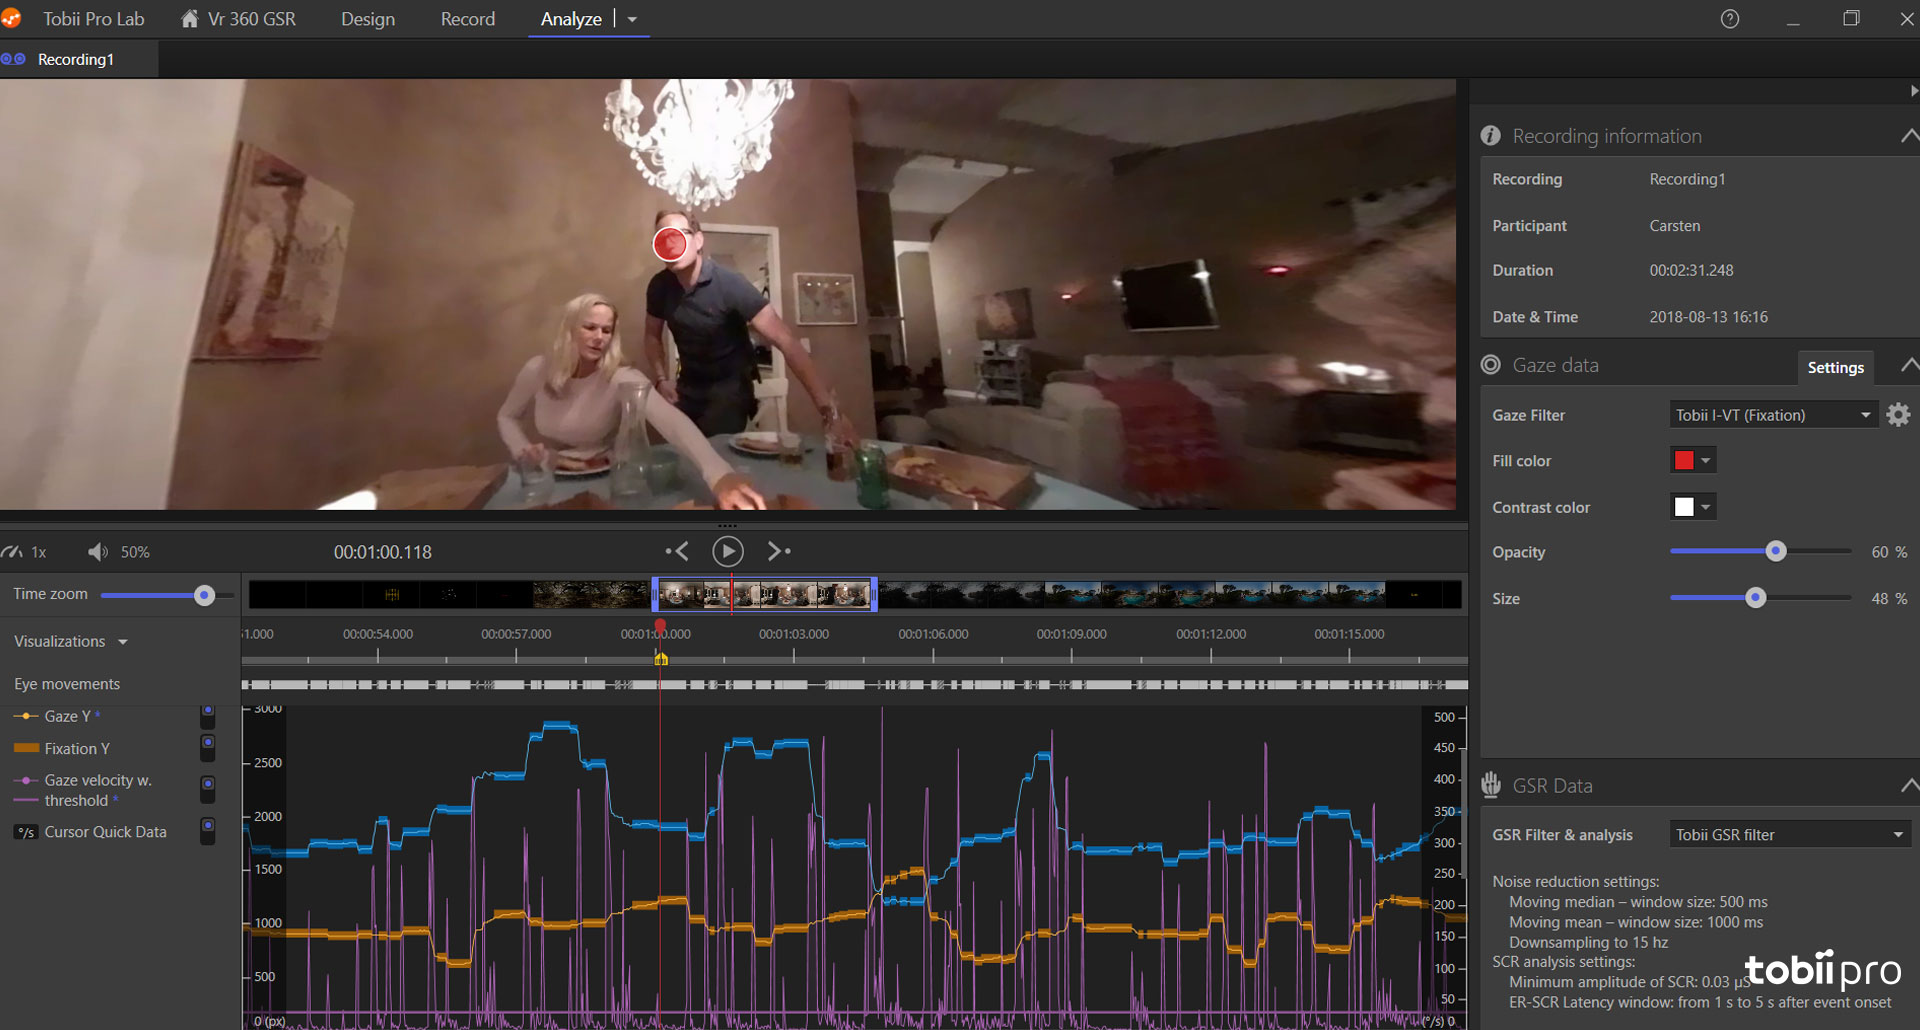
\includegraphics[width=1\textwidth]{images/02/tobiiprolab3.jpg}
    \caption{TODO, hľa softvér, nahradiť obrázkom, kde je zle vypočítaná oblasť pre reklamu.}
    \label{img:lab}
\end{figure}

% tensorboard https://medium.com/mlearning-ai/remote-tensorboard-viewing-on-your-local-browser-b0dc5c5a634a     and     https://pytorch.org/docs/stable/tensorboard.html

\section{Detektor reklám}

Narozdiel od predchádzajúcich YOLO verzií sa dá YOLOv8 nainštalovať a importovať priamo ako knižnica pre Python. Spolu s ňou sa do prostredia nainštalujú ďalšie dôležité knižnice ako matplotlib, opencv-python, scipy, torch, torchvision a iné. Trénovanie sa spúšťa pomocou jedného príkazu, kde argumenty špecifikujú základné parametre. Potrebné je nastaviť tri parametre: zdroj dát, počiatočné váhy a počet epoch. Zdroj bol je v našom prípade priečinok uložený na disku, ale ako zdroj sa dá použiť aj živý záznam z kamery alebo odkaz na video zverejnené na internete. Počiatočné váhy sa dajú stiahnuť z oficiálnej dokumentácie pre YOLOv8. Na výber je 5 modelov, ktoré sa líšia počtom parametrov, rýchlosťou a presnosťou. Ostatné parametre pre tréning majú hodnoty prednastavené podľa všeobecného odporúčania pre prvý tréning.

Dataset Mapillary Vistat má anotácie uložené vo formáte, ktorý nie je kompatibilný s formátom pre YOLO. Počas úpravy formátu sme zároveň vynechali obrázky, ktoré neobsahovali reklamu, čím sa počet obrázkov znížil na približne 20000 obrázkov. Pri prvom tréningu sme si všimli, že veľká chybovosť nastáva práve pri najmenšie označených reklamách. Najmenšie reklamy boli označené v takej diaľke, že by sa nedalo povedať, či sa vodič skutočne pozeral na reklamu, alebo na niečo iné. Preto sme z pôvodných dát vytvorili druhú verziu, kde sme ponechali len také obrázky, že reklamná plocha tvorí aspoň 0,1\% z obrázka. Dataset sa tým zmenšil takmer o polovicu. 

Pripravili sme ešte tretiu verziu dát, kde sme k vytriedeným dátam pridali 350 obrázkov s anotáciami reklám. Obrázky pochádzali z videí nahratých cez eyetracker, ktoré boli mimo experimentálnej trasy. 

Všetky tri verzie dát sme rozdelili na tri časti, v pomere 8:1:1 pre tréningovú, validačnú a testovaciu sadu. Postupne sme natrénovali tri modely, každý s inou verziou dát. Všetky modely mali pre tréning rovnako nastavené parametre, líšili sa jedine verziou dát. Počet epoch bol nastavený na 128, veľkosť dávky na 16 a ostatné boli ponechané s prednastavenými hodnotami. Najlepšie počiatočné váhy, s ktorými dokázal server pracovať mali označenie YOLOv8large.
\\
\begin{table}[ht]
\centering
\begin{tabular}{ |c c c c c|  }
\hline
model  &  presnosť & citlivosť & mAP50 & mAP50-95 \\
\hline
M1  & 0.473 & 0.352	& 0.327	& 0.195 \\
M2  & 0.659 & 0.565 & 0.656 & 0.467 \\
M3  & 0.623 & 0.575 & 0.636 & 0.456 \\
\hline
\end{tabular}
\caption{Výsledky prvých troch trénovaní. Modely sú označené číslom podľa verzie dát.}
\label{table:test1}
\end{table}

TODO Pri trénovaní sme mali k dispozícii výpis a tensorboard. bla bla
\\
\begin{figure}[ht]
    \centering
    
\includegraphics[width=1\textwidth]{images/02/placeholder.png}
    \caption{Výpis alebo tensorboard.}
    \label{img:lab}
\end{figure}

V tabuľke \ref{table:test1} je každý model otestovaný na príslušnej testovacej sade. Tým, že je každá sada iná, nemôžme povedať, ktorý model je najlepší. Pre lepšie otestovanie modelov sme si pripravili testovaciu vzorku obrázkov tvorenú zo snímok z experimentálneho merania. Vyhodnotenie modelov na testovacej vzorke v tabuľke \ref{table:test2} ukazuje, že model M3 dosahuje najlepšie výsledky a preto je najvhodnejší na pokračovanie v práci.
\\
\begin{table}[ht]
\centering
\begin{tabular}{ |c c c c c|  }
\hline
model & presnosť & citlivosť & mAP50 & mAP50-95 \\ 
\hline
M1  & 0.473	& 0.352	& 0.327	& 0.195 \\
M2  & 0.659 & 0.565 & 0.656 & 0.467 \\
M3  & 0.623 & 0.575 & 0.636 & 0.456 \\
\hline
\end{tabular}
\caption{Výsledky troch modelov na testovacej vzorke obrázkov.}
\label{table:test2}
\end{table}

% todo pridať obrázok, kde je graf z tréningu

% TODO skúsiť používať čo najviac slovenskú terminológiu
\subsection{Sledovanie reklám}

Na sledovanie reklám vo videách sa nám podarilo nájsť repozitár, v ktorom je možné vyskúšať viaceré sledovacie metódy. Vstupné video sa spracováva postupne snímok po snímku. Zo snímky sa pomocou modelu získajú detekcie, ktoré sú potom posielané na do zvolenej sledovacej metódy. Výstupom sledovacej metódy sú detekcie s priradenou referenciou.

Každá metóda má konfiguračný súbor, kde sa dá nastaviť viacero parametrov, ktoré ovplyvňujú sledovanie objektu. Dva najdôležitejšie parametre sú prahová hodnota pre detekciu objektu a prahová hodnota pre podobnosť objektov z predchádzajúcich snímok. Okrem toho sa dá nastaviť počet predchádzajúcich snímok, v ktorých sa porovnáva asociácia objektov, minimálny počet snímok na vytvorenie sekvencie a niekoľko ďalších špecifických pre jednotlivé metódy. Pre StrongSort je to napríklad maximálne vzdialenosť lokalizácie a pre OC-SROT asociačná funkcia.

S modelom M3 sme na vystrihnutej časti zo záznamu vyskúšali všetky metódy s rôznym nastavením parametrov. V tomto momente sme výsledky vyhodnotili iba pozorovaním, pretože sme nemali skutočne pravdivé údaje o výskyte reklám. Bolo vidno, že niektoré reklamy vôbec neboli objavené a pre niektoré chýbali detekcie len v určitých snímkach. Ďalšia chybovosť bola v priraďovaní referencií. Stávalo sa, že niektorá reklama dostala po čase priradenú inú referenciu ako na mala na začiatku. Opačný prípad bol, keď reklama viac nebola viditeľná a tá istá referencia bola priradená pre novú reklamu. Odhadli sme, že najlepšie výsledky dokázala metóda StrongSort, pretože na výstup uložila najmenší počet referencií a najviac označení

% todo zjednotiť slová video - nahrávka - experiment - záznam
\subsubsection{Pomocné dáta a model}

Na priblíženie sa ku skutočne pravdivým údajom sme sa rozhodli natrénovať nový pomocný model. Pre tento účel sme pripravili dataset, ktorý bol vytvorený zo snímok vystrihnutých z nahrávok experimentu. Reklamné plochy na vystrihnutých snímkam sme najskôr dali detegovať pomocou modelu M3. Získané označenia sme spolu s obrázkami pridali do webovej aplikácie Darwin v7labs \cite{v7}, kde sme následne opravili vzniknuté chyby z detekcie. Opraviť bolo treba približne každú druhý obrázok, ktorých spolu bolo takmer tisíc. Porovnanie výsledkov na pomocnom dataset pre 3. a 4. model \ref{table:test3}.
\\
\begin{table}[ht]
\centering
\begin{tabular}{ |c c c c c c| }
\hline
model & dáta & presnosť & citlivosť & mAP50 & mAP50-95 \\ 
\hline
M4 & testovacia sada & 0.473	& 0.352	& 0.327	& 0.195 \\
M3 & celý dataset & 0.659 & 0.565 & 0.656 & 0.467 \\
\hline
\end{tabular}
\caption{TODO, výsledky 3.}
\label{table:test3}
\end{table}

Pomocný model dosahoval pri sledovaní výrazne viac detekcií. Pre účely dosiahnuť čo najviac snímok s reklamou sme metódu StrongSort nastavili tak, aby mala čo najväčšiu citlivosť detekcie. Samozrejme sa tým znížila celková presnosť sledovania, ale to v podstate nebolo dôležité, pretože sme vedeli, že pred pokračovaním budeme potrebovať každú reklamu označiť rovnakou referenciou v každom videu, aby sme mohli analyzovať pohľady reklamu v každom videu.

Metódu s vysokou citlivosťou sme použili na detekciu reklám z každej nahrávky z merania. Museli sme opraviť dve chyby, falošne pozitívne detekcie a nesprávne priradenie referencie. Prakticky to znamenalo, že sme vytvorili kópie nahrávok, v ktorej boli vykreslené všetky detekcie s uvedenou referenciou. Pokiaľ išlo o správnu detekciu reklamy, tak sme priradenú referenciu nahradili poradovým číslom danej reklamy, ktorá bola rovnaké pre každé video. 

Dosiahli sme tým korektúru oboch chýb a získané označenia sme ďalej považovali za skutočne pravdivé údaje. Označenia sme zapísali do textového súboru vo formáte MOT pre každé video samostatne. Každá snímka, na ktorej sa nachádzala reklama bola zapísaná v samostatnom riadku s hodnotami pre poradie snímky, referencie reklamy, x a y súradnice ľavého horného rohu reklamy a pre rozmery reklamy.

\subsubsection{Testovanie sledovania}
V tomto momente sme už mohli vyhodnotiť úspešnosť sledovacích metód v porovnaní s pripravenými údajmi.

Na vyhodnotenie sledovania objektov, existuje viacero zaužívaných metrík. Dlhodobo používané metriky sú CLEAR MOT \cite{clear}, VACE \cite{vace}, IDF1 \cite{idf} a MOTA \cite{mota}. V roku 2020 bola publikovaná práca, v ktorej autori navrhli novú metriku so skratkou HOTA (Higher Order Tracking Accuracy) \cite{hota}. Práca dokazuje, že predchádzajúce metriky nedokážu zachytiť toľko informácií ako HOTA, ktorá je navyše pomerne intuitívna. Metrika HOTA sa dá rozložiť na viacero menších častí, čím sa dajú vyhodnotiť viaceré aspekty sledovania.

Localization measures the spatial alignment between one predicted detection and one ground-truth detection. Localization IoU (Loc-IoU) is typically used in many evaluation metrics to measure localization accuracy. It is calculated as the ratio of the overlap (intersection) between the two detections and the total area covered by both of them (union). As can be seen, when the Loc-IoU score here increases, the predicted and ground-truth detections are better spatially aligned and the localization is improved.

We can measure the overall Localization Accuracy (LocA) by averaging the Loc-IoU over all pairs of matching predicted and ground-truth detections in the whole dataset (we describe below how we obtain these matches):

\begingroup
\large
\begin{equation}
LocA = \frac{A}{B}
\label{e:DetRe}
\end{equation}
\endgroup
\\
Citlivosť a presnosť detekcie (DetRe a DetPr) je definovaná rovnakým spôsobom ako pri vyhodnocovaní detektora. Detekcie, ktoré sú zhodné so skutočne pravdivým označením sa volajú skutočne pozitívne (TP) a detekcie, ktoré nie sú zhodné sa volajú falošne pozitívne (FP). Na základe toho sa dajú sformulovať tri rovnice. 
Rovnica \ref{e:DetRe} opisuje koľko TP detekcií bolo nájdených zo všetkých skutočne pravdivých označení, rovnica \ref{e:DetPr} opisuje úspešnosť pravdivosti pre TP detekcie a napokon rovnica \ref{e:DetA} celkovú presnosť detekcií.

\begingroup
\large
\begin{equation}
DetRe = \frac{A}{B}
\label{e:DetRe}
\end{equation}

\begin{equation}
DetPr = \frac{A}{B}
\label{e:DetPr}
\end{equation}

\begin{equation}
DetA = \frac{A}{B}
\label{e:DetA}
\end{equation}
\endgroup
\\
% https://jonathonluiten.medium.com/how-to-evaluate-tracking-with-the-hota-metrics-754036d183e1
Asociácia meria ako dobre sa podarilo spojiť detekciu s referenciou.  The intersection between two tracks can be measured as the number of True Positive matches between the two tracks, we call these True Positive Associations (TPA). Any remaining detections in the predicted track (which are either matched to other ground-truth tracks or none at all) are False Positive Associations (FPA) and any remaining detections in the ground-truth track False Negative Associations (FNA). The Association IoU (Ass-IoU) can then be calculated in a similar way as seen previously.

\begingroup
\large
\begin{equation}
AssRe = \frac{A}{B}
\label{e:AssRe}
\end{equation}

\begin{equation}
AssPr = \frac{A}{B}
\label{e:AssPr}
\end{equation}

\begin{equation}
AssA = \frac{A}{B}
\label{e:AssA}
\end{equation}
\endgroup
\\
We can see a visual example of the definitions TPA, FNA and FPA below. The red square indicates the matched TP pair of a prediction and ground-truth detection, for which we want to find an association score. In order to measure how good the temporal association aligns between these detections, we find all the detections in these two tracks which match between these tracks (TPAs in green) and all the detections where they don’t match (FPAs in yellow and FNAs in brown).

% A visual explanation of the concepts of TPA, FPA and FNA. The different TPAs, FPAs and FNAs are highlighted for the TP of interest c. The TPAs (green) for c (red) are the matches which have the same prID and the same gtID. The FPAs have the same prID but either a different or no gtID. The FNAs have the same gtID but either a different or no prID. In the diagram, c has five TPAs, four FPAs and three FNAs. Conceptually these concepts are trying to answer the question: For the matched TP c, how accurate is the alignment between the gtTraj for this TP (large dark blue circles) and the prTraj for this TP (small black circles).

% https://arxiv.org/pdf/2009.07736.pdf 

\begin{figure}[ht]
    \centering
    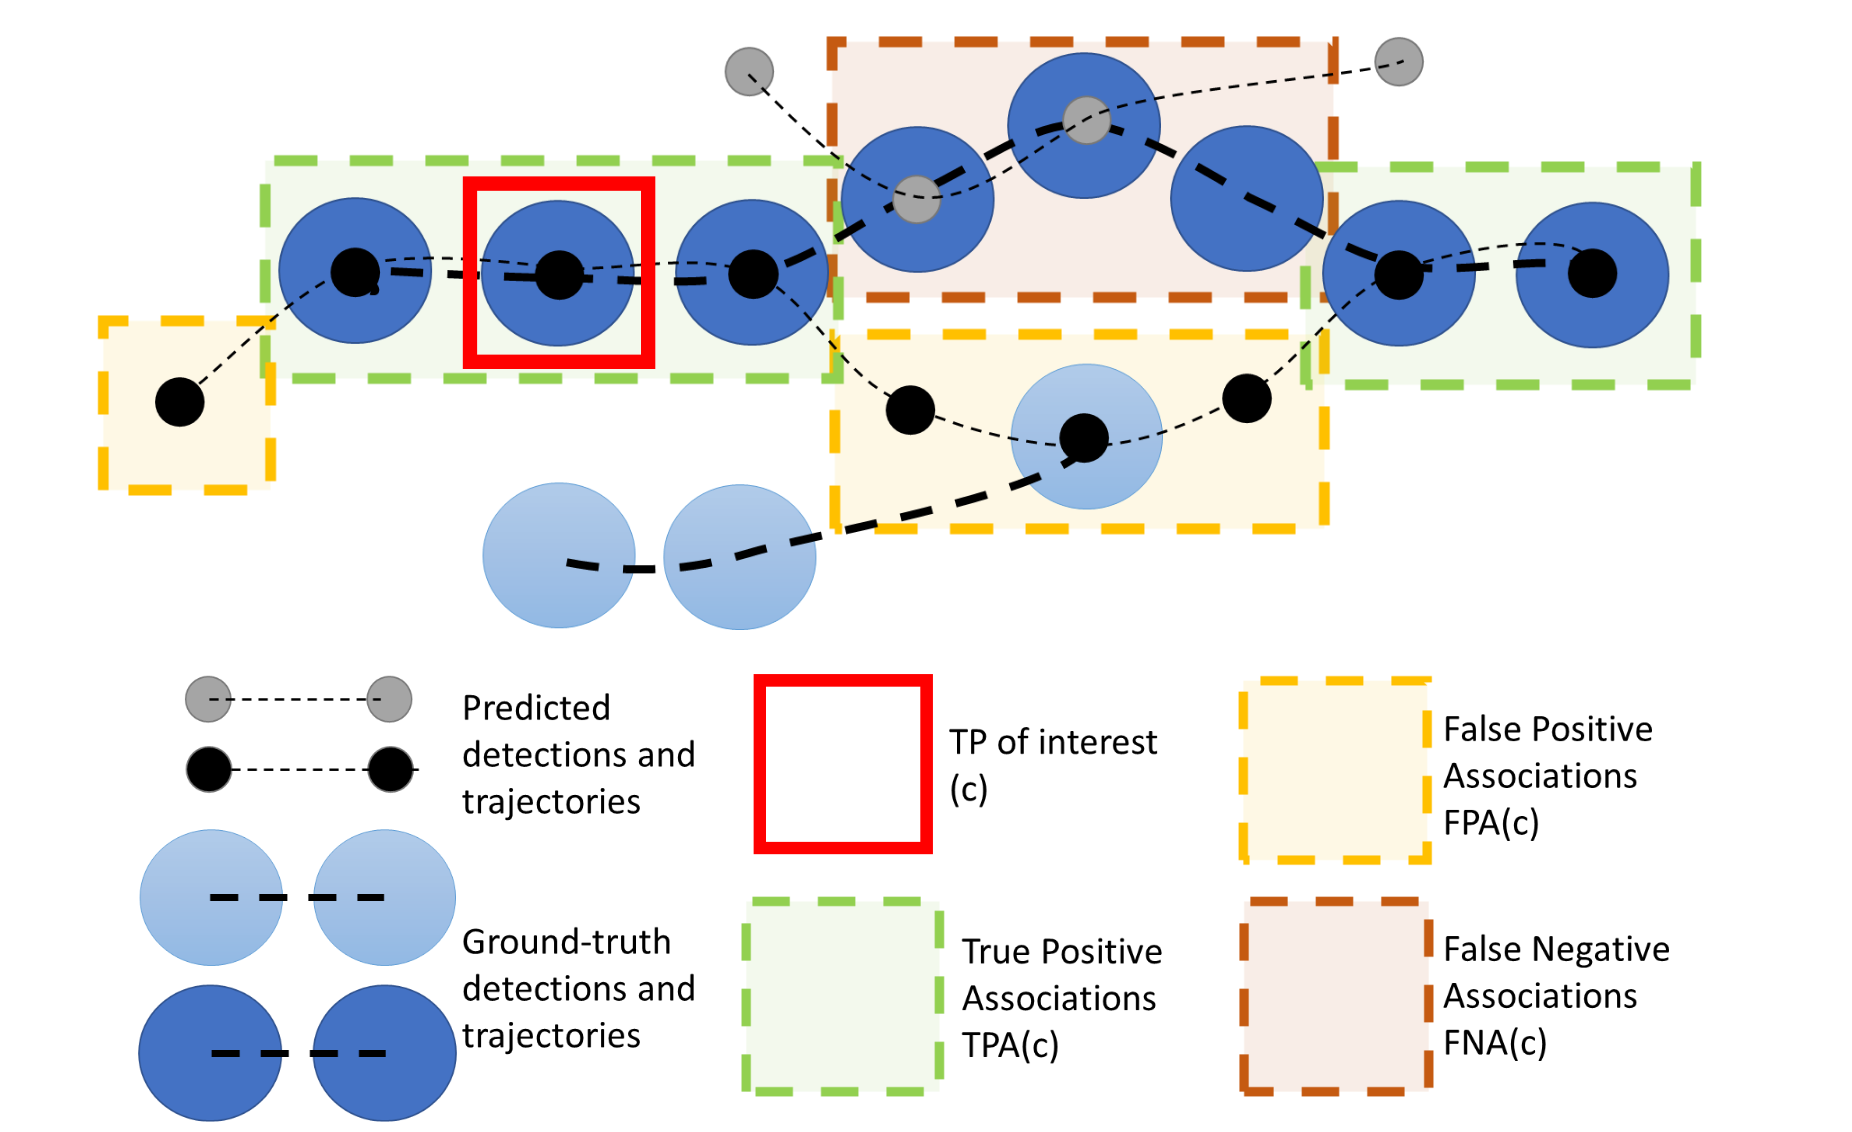
\includegraphics[width=1\textwidth]{images/T/explanation.png}
    \caption{.}
    \label{img:road}
\end{figure}

Nakoniec kompozíciou detekcie a asociácie je vypočítaná hodnota HOTA \ref{e:hota}. TODO We see that HOTA is equal to the geometric mean of a detection score and an association score. This formulation ensures that both detection and association are evenly balanced, unlike many other tracking metrics, and that the final score is somewhere between the two. It also ensures that both the detection score and association score have the same structure.
\begingroup
\large
\begin{equation}
LocA = \frac{A}{B}
\label{e:hota}
\end{equation}
\endgroup
\\
Každá sledovacia metóda bola spustená viackrát s iným nastavením. Najlepšie výsledky pre každú metódu sú zapísané v tabuľke \ref{table:hota1}. Po vyhodnotení vidno, že náš odhad najlepšej metódy sa potvrdil.
\\
\begin{table}[ht]
\centering
\begin{tabular}{|c c c c c c c c c|} 
 \hline
TODO metóda & HOTA & DetPr & DetRe & DetA & AssPr & AssRe & AssA & LocA \\ [0.5ex] 
 \hline
strongsort & 39.152 & 63.357 & 54.578 & 42.673 & 70.841 & 42.888 & 35.937 & 88.932 \\ [0.1ex]
deep & 39.152 & 63.357 & 54.578 & 42.673 & 70.841 & 42.888 & 35.937 & 88.932 \\ [0.1ex]
oc & 37.936 & 58.479 & 54.554 & 40.455 & 74.731 & 42.579 & 35.638 & 88.581 \\ [0.1ex]
byte & 27.760 & 37.434 & 34.147 & 22.085 & 57.887 & 47.258 & 34.957 & 88.027 \\ [0.1ex]
bot & 27.141 & 40.139 & 38.162 & 24.812 & 40.389 & 56.746 & 29.729 & 87.301 \\ [0.1ex]
 \hline
\end{tabular}
\caption{TODO, výsledky 4.}
\label{table:hota1}
\end{table}
\\
TODO We can see how well methods perform in each of the dimensions of detection (x-axis) and association (y-axis) separately, with the curves in the background showing how the overall HOTA score increases as both detection and association scores increase. We can go further than just comparing detection and association. Because they are both naturally decomposable into one component.
\begin{figure}[ht]
    \centering
    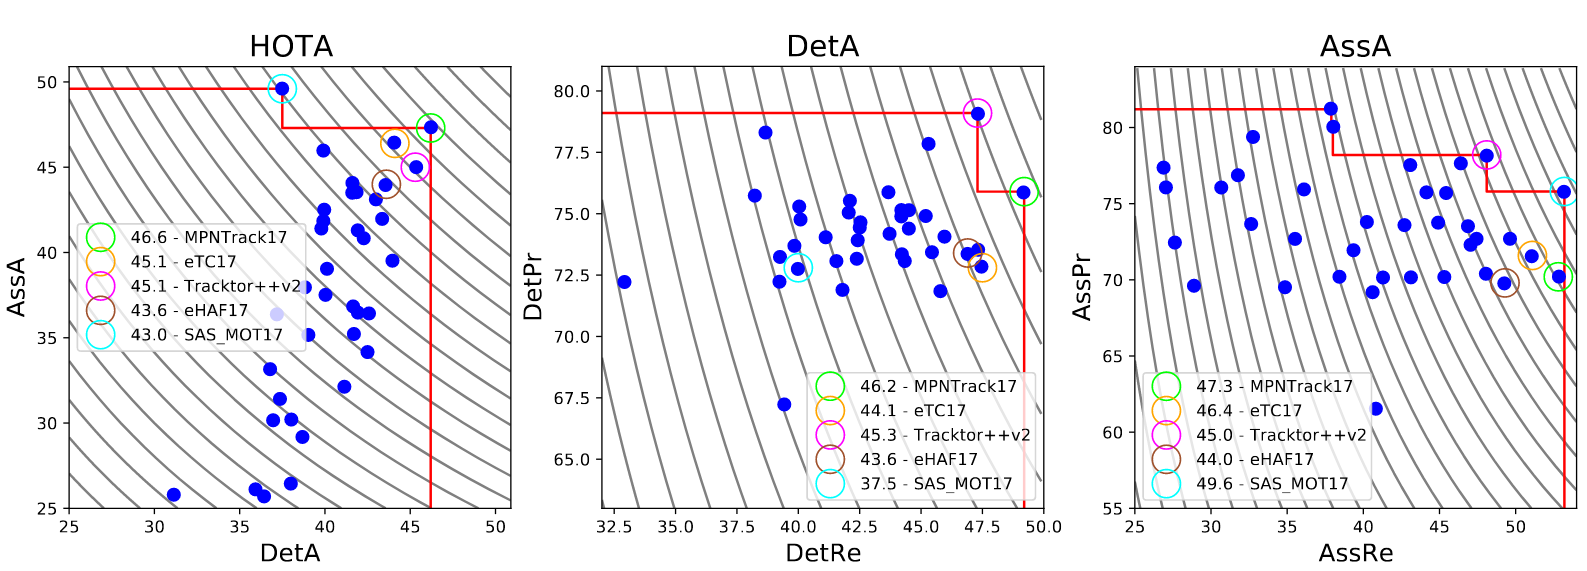
\includegraphics[width=1\textwidth]{images/T/compare.png}
    \caption{.}
    \label{img:road}
\end{figure}

TODO Tu je vizualizácia sledovania reklám z videa. Na pravej strane obrázka je metóda X a na ľavej Y. Snímky sú v tomto prípade zachytené každých 10 snímok a vidíme, že metóda Y nepriradila referenciu po oklúzii správne.
\begin{figure}[ht]
    \centering
    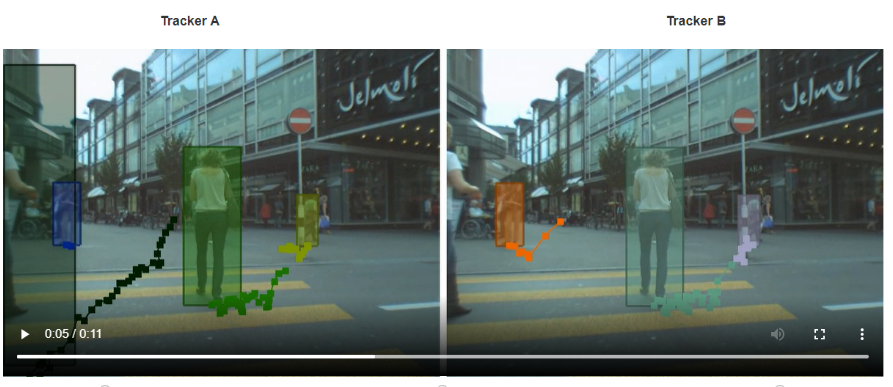
\includegraphics[width=1\textwidth]{images/T/vs.png}
    \caption{.}
    \label{img:road}
\end{figure}

\subsection{Významnosť reklám}
% todo pozrieť skloňovanie pre snímku - ženský rod
Potom čo sa nám podarilo získať informácie, na ktorých snímkach sa nachádza reklama, sme mohli začať analyzovať pohľady vodiča. V tomto bode sme zistili, že pohľady boli zaznamenané v počte 50 snímok za sekundu, kým video bolo nahrávané v počte 25 snímok za sekundu. To znamená, že pokiaľ bol pohľad zaznamenaná bez straty mali sme pre každú snímku z videa dva pohľady. Kvôli nedokonalému nahrávaniu na niektorých snímkach chýbal jeden, či dokonca oba pohľady. Pokiaľ sme pre snímok zaznamenali chýbajúci pohľad, vypočítali sme jeho predikciu pomocou. Predikciu sme počítali pomocou dvoch predchádzajúcich pohľadov. Pre výpadok pohľadu na viac ako dve snímky sme predikciu nepočítali a snímok sme z analýzy vynechali.

To či sa vodič pozrel na reklamy sme vyhodnotili vypočítaním prieniku označenej reklamy so zaznamenanou súradnicou s polomerom 20 pixlov. Dokopy bolo na zvolenej trase nájdených 145 reklám, ktoré sa podľa počtu prienikov rozdelili do štyroch kategórií. V tabuľke \ref{table:cat} je pre každú kategóriu zapísané časové rozmedzie korešpondujúce počtu snímok s prienikom, počet reklám vyhodnotených do príslušnej kategórie a priemerný počet účastníkov, ktorý sa na reklamu danej kategórie pozreli.
% todo pridať obrázok, kde je fixácia
\\
\begin{table}[ht]
\centering
\begin{tabular}{|c c c c|}
 \hline
 kategória &	rozmedzie &	počet reklám &	počet účastníkov \\ [0.5ex] 
 \hline
slabá &	0 ms &	27 &	- \\ [0.1ex]
nízka &	1-249 ms &	66 &	2.95 \\ [0.1ex]
stredná &	250-499 ms &	18 &	5.11 \\ [0.1ex]
vysoká &	500+ ms &	3 &	2 \\ [0.1ex]
 \hline
\end{tabular}
\caption{TODO, výsledky 5.}
\label{table:cat}
\end{table}

\subsection{Klasifikácia reklamy}


% optimalizácia hyperparametre, Under/over-fitting
% augmentacia pred trenovanim, pri testovani (Test time augmentation)
% porovnanie precision a recall pre detector vs tracker

% can object tracking improve object detection?

% Yes, object tracking can improve object detection. Object tracking can be used to refine the object detection process by providing additional information about the location and movement of objects in a video stream. By tracking objects across multiple frames, object tracking algorithms can help to reduce false positives and false negatives in the object detection process. For example, if an object detection algorithm detects an object in one frame but fails to detect it in the next frame, an object tracking algorithm can use the object's previous position and movement to predict its location in the current frame. This can help to reduce the number of false negatives and improve the accuracy of the object detection algorithm. Additionally, object tracking can be used to filter out false positives in the object detection process. By tracking an object across multiple frames, an object tracking algorithm can verify that the object is indeed present and is not just a false positive detection. This can help to improve the precision of the object detection algorithm. Overall, object tracking and object detection are complementary techniques that can be used together to improve the accuracy and robustness of computer vision systems.


% porovnať chybosť kategorizácie, kebyže sa to počíta zo standardného modelu

% porovnať chybosť klasifikácie, kebyže sa to počíta zo standardného modelu